\documentclass{article}
\usepackage[a4paper, tmargin=1in, bmargin=1in]{geometry}
\usepackage[utf8]{inputenc}
\usepackage{graphicx}
\usepackage[justification=centering]{caption}

% \usepackage{parskip}
\usepackage{pdflscape}
\usepackage{listings}
\usepackage{hyperref}
\usepackage{caption}
\usepackage{subcaption}
\usepackage{float}
\usepackage{amsmath}
\DeclareMathOperator*{\argmax}{\arg\!\max}
\title{CS 747 : Foundations of Intelligent Learning Agents Assignment 4}
\author{Arka Sadhu - 140070011}
\date{\today}

\begin{document}
\maketitle

\section{Problem Statement}
In the assignment we are asked to use value function approximation for a specific MDP called the Baird's counterexample. There are a total of 6 states with 5 of those going to the $6^{th}$ state with probability 1 and the $6^{th}$ state self-looping with probability 0.99 and terminating with probability $0.01$. The rewards for all the transitions are zero. The functional approximation is chosen as follows:

\[%
F= \begin{bmatrix}%
2&0&0&0&0&0&1\\%
0&2&0&0&0&0&1\\%
0&0&2&0&0&0&1\\%
0&0&0&2&0&0&1\\%
0&0&0&0&2&0&1\\%
0&0&0&0&0&1&2%
\end{bmatrix}%
\]

The initial weight vector for this experiment is taken as all weights as 1. That is

\[%
w= \begin{pmatrix}%
1\\%
1\\%
1\\%
1\\%
1\\%
1\\%
1%
\end{pmatrix}%
\]

The value function vector is given as $V = Fw$

\section{Experiment 1}
For Experiment 1 we are required to choose the one of the six states at random and update the weight values according to the TD(0) update which includes full bootstrapping. The TD(0) updates are made N times where N is given by the user. For each update the value function of each state is noted and the corresponding graph is plotted. X axis is the number of updates and y-axis is the value function

\begin{figure}[H]
  \centering
  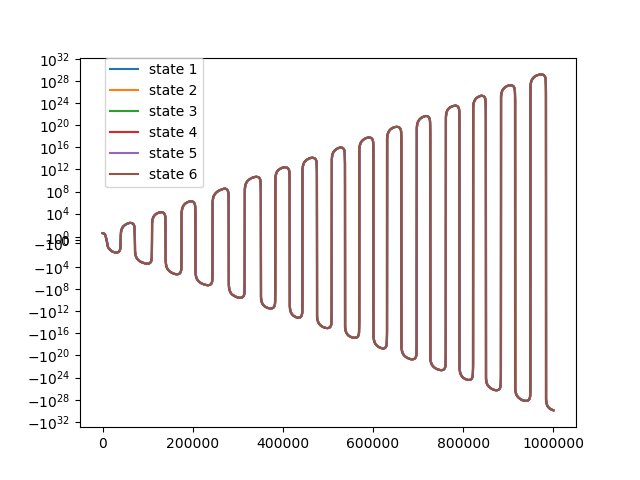
\includegraphics[scale=0.5]{images/exp1}
  \caption{Experiment 1 graph}
  \label{fig:ex1}
\end{figure}
Even though separate lines have been drawn for each state, since the values are so large, it is difficult to distinguish between the values. Though it is noted that the value function of state 6 is different from the other states. In expectation the value function of the other states (states 1-5) follows the same trajectory because states 1-5 are symmetric in their features and initial weight values.

Observations:
\begin{itemize}
\item We note the the value function doesn't converge to the correct value of being 0 at every state. In fact it diverges to infinity.
\item Also the divergence is somewhat peculiar because it is sometimes positive and sometimes negative often going to extreme in both the cases.
\item At the start the value function decreases and then increases and then continues this in an alternating manner.
\item The increase or decrease when going from positive to negative is quite rapid followed by a linear increase or decrease in the value function.
\item Moreover the interval for linear increase and decrease as well as the rapid increase and decrease is periodic.
\item $V(state6)$ increases and decreases faster than the other states.
\item A few experiments with differing weights also lead to divergence.
\item Starting with initial weights of 0 is the only one which doesn't diverge and stays exactly as it is.
\end{itemize}

Inferences:
\begin{itemize}
\item The main reason for the divergence is that even though the probability of staying at state 6 is much higher than any of the other states 1-5, when selecting a state in a round robin manner we are choosing each of the 6 states equally likely and therefore the update of the state 6 is not updated as often it should have been. As a result this leads to divergence.
\item We recall the update of weights for the TD(0) which is:
  $$\delta = r + \gamma * V(s') - V(s)$$
  $$w = w + \alpha * \delta * x(s)$$
  Here $\gamma=0.99$ is the discount factor and $\alpha$ is the learning rate and $x(s)$ is the feature vector of state $s$ and $V(s)$ is the value function of state $s$.
\item Since the reward for each transition is exactly $0$ we have $\delta < 0$ at the start. For the states 1-5 we will then have the weights corresponding to that state decrease initially. For state 6, we almost always have $\delta < 0$ but nearly 0 and sometimes much less than 0 (when terminating). As a result all the keep on decreasing. Initially $\delta$ is very close to 0 which is the cause of the slow start.
\item Since state 6 depends more on $w(7)$ than others and since $w(7)$ is being altered by every iteration (even by states 1-5) as a result of which it becomes negative earlier than the other states, we note that state 6 is the first to become negative.
\item It is also important to note that state 6 contributes quite less to decrease of $w(7)$ because of $\delta$ being quite small for its iteration.
\item The decreasing trend of weights continues until for one of the states the $\delta$ becomes positive. The dynamics can be followed by looking at the $\delta$ for two states. For state 1 it will be
  $$\delta = \gamma ( w(6) + 2 w(7)) - (2w(1) + w(7))$$
  Initially $\delta$ is nearly zero (as pointed out earlier). Since $w(7)$ update happens 5 times for states 1-5, and $w(1)$ effectively happens twice for update of state 1, it is easy to see that $w(7)$ will decrease at a much faster rate than $w(1)$ and as such $\delta$ will remain negative. But this would suggest it would go on decreasing and here we see that there is a catch. The $\delta$ for state 6 is
  $$\delta = (\gamma - 1)(w(6) + 2w(7))$$
  If the next state is terminal then the update equation becomes:
  $$\delta = -(w(6) + 2w(7))$$
  We note that after some time, $w(6) + 2w(7)$ becomes negative leading to a positive $\delta$ for state 6 and therefore state 6 now increases $w(7)$. Occassionally when it reaches the terminal state the increase in $w(7)$ is much faster
\item Now that $w(7)$ is increasing it will ultimately lead to $\delta$ for state 1 to become positive, and then $w(1)$ will be increased. This again happens till value function for state 6 stays negative.
\item This interval is more or less a constant because the occassional termination in expectation averages out and we are using a constant learning rate. This is the period where the value function increase/decrease is more or less linear.
\item Again when the value function changes sign, $\delta$ for state 6 changes sign, leading to changing the direction of $w(7)$ which will in effect lead to change in sign of $\delta$ for state 1 after some iterations. And hence the pattern continues. Everything stated for state 1 is equally applicable for states 1-5 equally.
\item The divergence is precisely because $w(7)$ gets  more updates from other states than state 6 which should ideally act as a feedback.
\end{itemize}

\section{Experiment 2}
In this experiment we are required to follow the MDP instead of choosing the states in a round-robin manner. We are required to use TD($\lambda$) updates for $\lambda$ = \{0, 0.2, 0.4, 0.6, 0.8, 1\}. For each lambda we are required to get the average of all the value functions of the states for that particular iteration. The corresponding plot is shown here:
\begin{figure}[H]
  \centering
  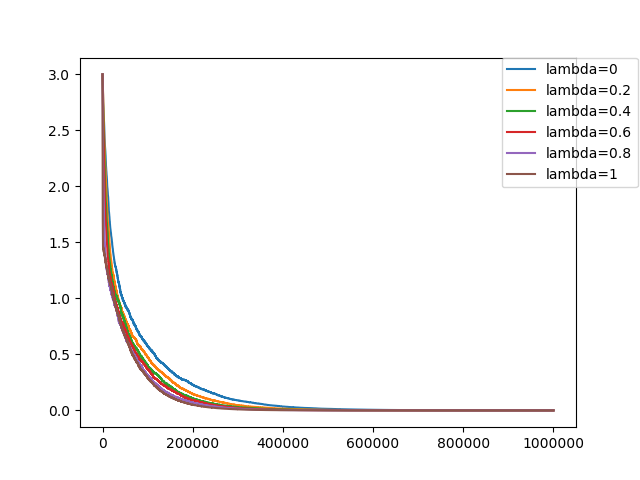
\includegraphics[scale=0.5]{images/exp2}
  \caption{Experiment 2 plot}
  \label{fig:ex2}
\end{figure}

The x-axis is the number of updates, while y-axis is the corresponding value function averaged over the states.

Observations and Inferences:
\begin{itemize}
\item The first thing to note is that the value functions are converging to zero which is exactly what we want. It doesn't diverge like in the first experiment. The main reason for this is that state 6 is able to prevent the weight $w(7)$ from blowing up because of other states, since it is able to make more number of updates than the other states.
\item There is a stark variation due to the influence of $\lambda$. For lower value of $\lambda$ the value function converges slower than that for higher $\lambda$ value. This is because for $\lambda = 0$ it doesn't weigh in more than one reward whereas for higher $\lambda$ it sees the whole episode before making any decision. This leads to fastest convergence of TD(1).
\item It is also noted that for that the asymptotic characteristics also follow the same pattern that is TD(1) is converges to a better optimal than TD(0). This can be seen here:
  \begin{figure}[H]
    \centering
    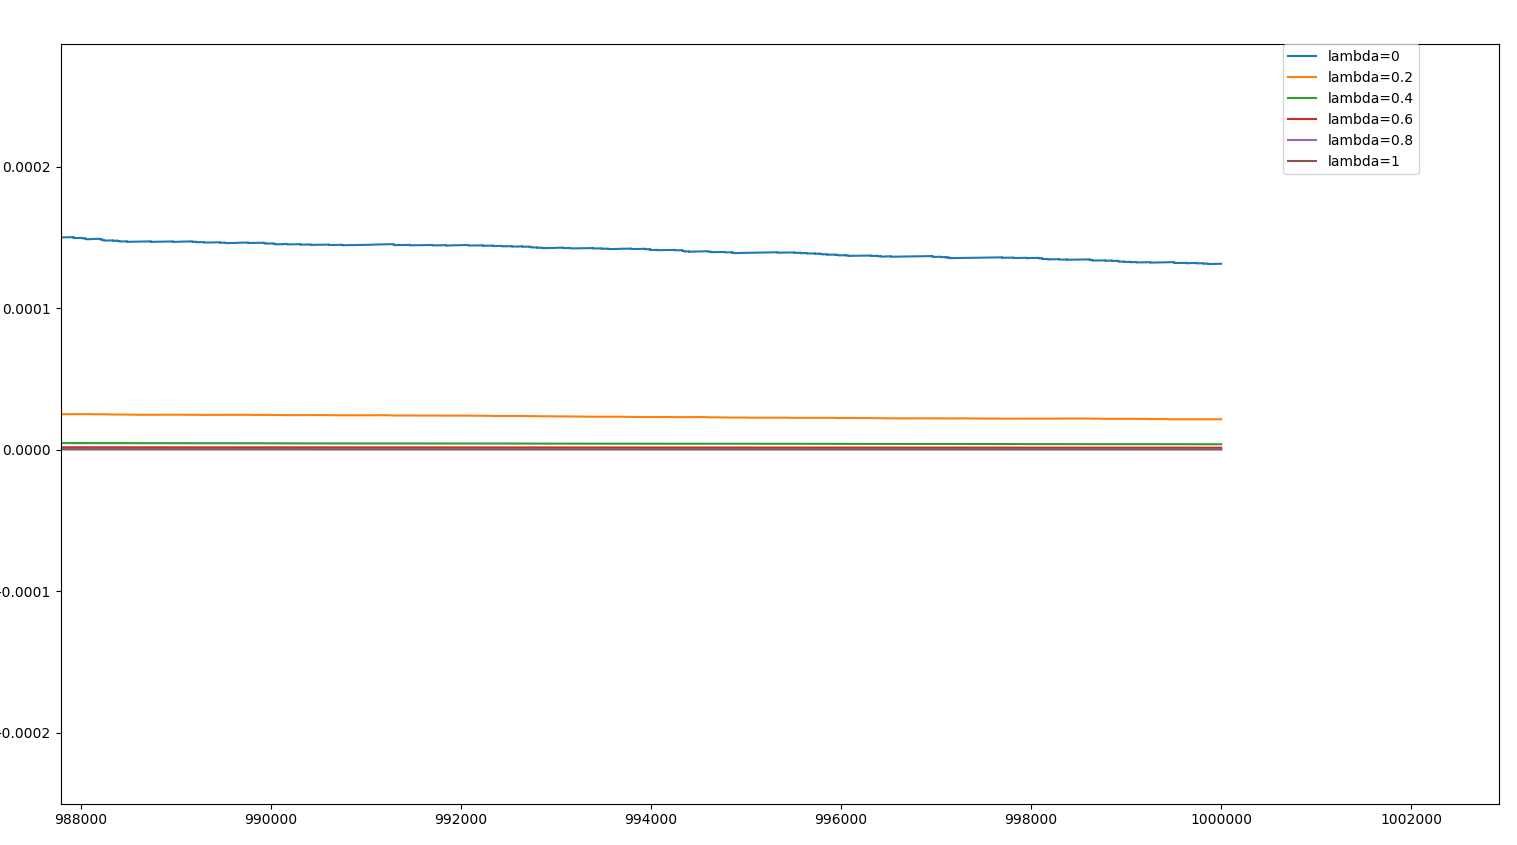
\includegraphics[scale=0.25]{images/exp22}
    \caption{Experiment asymptotic characteristics}
    \label{fig:ex22}
  \end{figure}
\end{itemize}
The reason for this behaviour is also the same. TD(1) is the only one guarenteed to converge to the best approximation, while others only come to small neighborhood of it.

\section{Experiment 2 with different Initial Weights}
It is easily seen that for different initial weights the weights do not converge to the same weights for TD(0). The value function with any weights tends to all zero but since we are using TD(0) we are only guarenteed to converge to a very small neighborhood of 0 but not exactly. Therefore observation at any finite time we will not get exact same value function. After infinite time we can expect convergence.

The different weights is simply because there are multiple weights which result in the same value functions. So the sequence of weights can converge to any of the weights which result in the correct value function. On careful observation it can be seen it will be 1-D span of a vector to which it should converge. (1-D span which is precisely the null space of the feature matrix).
\end{document}